% ============================================================
%  EE-559 Poster — Watch. Listen. Read.
%  Authors: Youssef Dib, Kevin Abou Jaoude, Rami Aschkar
%  Group 07 · EPFL EE-559, Spring 2026
%
%  Compile: pdflatex poster.tex  (twice)
%  Requires: a0poster, tcolorbox, tikz — all in TeX Live / Overleaf.
%  Print: A0 portrait, 100% scale.
%
%  Quick editing guide:
%    Numbers in tables  → search \% and change the value
%    Section text       → inside \begin{pbox}{Title} … \end{pbox}
%    Colors             → \definecolor block near the top
%    Stat strip numbers → search "STAT STRIP"
%    Architecture       → tikzpicture under "ARCHITECTURE"
% ============================================================
\documentclass[a0paper,portrait,final]{a0poster}

\usepackage[left=22mm,right=22mm,top=14mm,bottom=8mm]{geometry}
\usepackage[T1]{fontenc}
\usepackage[utf8]{inputenc}
\usepackage{helvet}
\renewcommand{\familydefault}{\sfdefault}

\usepackage{xcolor}
\usepackage[most]{tcolorbox}
\usepackage{tikz}
\usetikzlibrary{arrows.meta,positioning}
\usepackage{graphicx}
\usepackage{booktabs}
\usepackage{array}
\usepackage{colortbl}
\usepackage{microtype}
\usepackage{enumitem}
\usepackage{ragged2e}

\pagestyle{empty}

% ─────────────────────────────────────────────────────────
%  COLORS
% ─────────────────────────────────────────────────────────
\definecolor{epflred}   {RGB}{196, 30,  26}   % EPFL brand red
\definecolor{darkbg}    {RGB}{ 26, 26,  26}   % stat strip
\definecolor{fusionrow} {RGB}{254,242, 242}   % table fusion row tint
\definecolor{keyobsbg}  {RGB}{245,247, 250}   % key obs background
\definecolor{videobg}   {RGB}{219,234, 254}   % CLIP encoder tint
\definecolor{audiobg}   {RGB}{220,252, 231}   % wav2vec encoder tint
\definecolor{textpurbg} {RGB}{237,233, 254}   % RoBERTa encoder tint
\definecolor{warnred}   {RGB}{248,113, 113}   % bias callout text
\definecolor{dsgray}    {RGB}{245,245, 245}   % dataset stat card bg

% ─────────────────────────────────────────────────────────
%  BOXES  (tcolorbox styles)
% ─────────────────────────────────────────────────────────

% Standard poster section: red header bar, white body
\newtcolorbox{pbox}[1]{
  enhanced, breakable,
  title        = {\LARGE\bfseries\color{white} #1},
  colbacktitle = epflred,
  coltitle     = white,
  colback      = white,
  colframe     = epflred!20,
  boxrule      = 0.4pt,
  arc          = 2mm,
  top          = 4mm, bottom = 4mm,
  left         = 5mm, right  = 5mm,
  toptitle     = 3mm, bottomtitle = 3mm,
  attach boxed title to top left,
  boxed title style = {
    sharp corners, colback=epflred, colframe=epflred, arc=0mm
  },
}

% Dark box (bias callout)
\newtcolorbox{darkbox}{
  enhanced,
  colback  = darkbg,
  colframe = darkbg,
  arc      = 2mm,
  top = 5mm, bottom = 5mm,
  left = 5mm, right = 5mm,
}

% Left-accented box (key observations)
\newtcolorbox{obsbox}{
  enhanced,
  colback  = keyobsbg,
  colframe = epflred,
  leftrule = 5pt,
  rightrule= 0pt,
  toprule  = 0pt,
  bottomrule=0pt,
  arc      = 0mm,
  top = 5mm, bottom = 5mm,
  left = 5mm, right = 5mm,
}

% ─────────────────────────────────────────────────────────
%  SHORTCUTS
% ─────────────────────────────────────────────────────────
\newcommand{\clabel}[1]{\textcolor{epflred}{\textbf{#1}}}
\newcommand{\vtag}{\colorbox{videobg}  {\large\bfseries\textcolor{blue!80!black}{see}}}
\newcommand{\atag}{\colorbox{audiobg}  {\large\bfseries\textcolor{green!60!black}{hear}}}
\newcommand{\ttag}{\colorbox{textpurbg}{\large\bfseries\textcolor{purple!80!black}{read}}}

% ─────────────────────────────────────────────────────────
\begin{document}

% ═════════════════════════════════════════════════════════
%  TOP RED BAND
% ═════════════════════════════════════════════════════════
\noindent\colorbox{epflred}{\makebox[\dimexpr\textwidth][l]{\hfill}}%
\vspace{-2mm}

% ═════════════════════════════════════════════════════════
%  HEADER
% ═════════════════════════════════════════════════════════
\noindent
\begin{minipage}[b]{0.80\textwidth}
  {\VERYHuge\bfseries\itshape Watch.\;
   \textcolor{epflred}{Listen.}\; Read.}\\[3mm]
  {\LARGE Can a computer catch hate speech better by
   \textbf{seeing}, \textbf{hearing}, and \textbf{reading}
   a video all at once?}\\[4mm]
  {\Large\bfseries Youssef Dib \quad Kevin Abou Jaoude \quad Rami Aschkar
   \quad \textcolor{epflred}{· Group 07}}
  \hfill
  {\large\color{gray} EE-559 Deep Learning · EPFL, Spring 2026}
\end{minipage}%
\hfill
\begin{minipage}[b]{0.18\textwidth}
  \raggedleft
  {\VeryHuge\bfseries\textcolor{epflred}{EPFL}}
\end{minipage}

\vspace{3mm}
\noindent{\color{epflred}\rule{\textwidth}{2.5pt}}
\vspace{2mm}

% ═════════════════════════════════════════════════════════
%  STAT STRIP  — edit numbers here
% ═════════════════════════════════════════════════════════
\noindent\colorbox{darkbg}{%
  \begin{minipage}[c]{\dimexpr\textwidth\relax}%
    \vspace{5mm}
    \centering
    % card 1
    \begin{minipage}[c]{0.23\textwidth}\centering
      \textcolor{epflred}{\huge\bfseries 83.5\%}\\[2mm]
      \textcolor{white}{\large Accuracy}\\[1mm]
      \textcolor{gray}{\normalsize fusion model}
    \end{minipage}%
    \hspace{0.01\textwidth}%
    \textcolor{gray!40}{\rule{0.5pt}{20mm}}%
    \hspace{0.01\textwidth}%
    % card 2
    \begin{minipage}[c]{0.23\textwidth}\centering
      \textcolor{epflred}{\huge\bfseries 82.4\%}\\[2mm]
      \textcolor{white}{\large Macro F1 Score}\\[1mm]
      \textcolor{gray}{\normalsize balanced hate/non-hate}
    \end{minipage}%
    \hspace{0.01\textwidth}%
    \textcolor{gray!40}{\rule{0.5pt}{20mm}}%
    \hspace{0.01\textwidth}%
    % card 3
    \begin{minipage}[c]{0.23\textwidth}\centering
      \textcolor{epflred}{\huge\bfseries 87.3\%}\\[2mm]
      \textcolor{white}{\large AUROC}\\[1mm]
      \textcolor{gray}{\normalsize ranking quality}
    \end{minipage}%
    \hspace{0.01\textwidth}%
    \textcolor{gray!40}{\rule{0.5pt}{20mm}}%
    \hspace{0.01\textwidth}%
    % card 4
    \begin{minipage}[c]{0.23\textwidth}\centering
      \textcolor{epflred}{\huge\bfseries +5\,pt}\\[2mm]
      \textcolor{white}{\large AUROC gain}\\[1mm]
      \textcolor{gray}{\normalsize fusion vs.\ text-only}
    \end{minipage}
    \vspace{5mm}
  \end{minipage}%
}

\vspace{6mm}

% ═════════════════════════════════════════════════════════
%  TWO-COLUMN BODY
%  Change 0.465 / 0.465 to adjust column widths.
%  Gap = \textwidth - left_col - right_col = 7% of textwidth.
% ═════════════════════════════════════════════════════════
\noindent
\begin{minipage}[t]{0.465\textwidth}

  % ────────────────────────────────────────
  %  THE PROBLEM
  % ────────────────────────────────────────
  \begin{pbox}{The Problem}
    Every day, thousands of videos are posted online targeting people
    based on race, religion, or identity.
    Detecting this \emph{automatically} is hard --- the hate is not
    always in the words alone.
    Sometimes you need to
    \vtag{} the imagery,
    \atag{} the tone of voice, \textbf{and}
    \ttag{} what is being said
    to tell hate from satire or critical commentary.

    \vspace{4mm}
    \clabel{Our question:}
    Does a model using \emph{all three signals at once}
    outperform models that use only one?
    And does it work equally well for different target communities?
  \end{pbox}

  \vspace{5mm}

  % ────────────────────────────────────────
  %  DATASET
  % ────────────────────────────────────────
  \begin{pbox}{Dataset --- HateMM}
    \textbf{HateMM} (Das et al., ICWSM 2023), released under CC~BY~4.0.
    Real BitChute videos, each manually labelled hateful or non-hateful
    with the targeted community noted.

    \vspace{5mm}
    % Three stat cards
    \noindent
    \begin{minipage}[t]{0.31\linewidth}\centering
      \colorbox{dsgray}{\begin{minipage}[c][22mm][c]{0.9\linewidth}
        \centering
        \textcolor{epflred}{\LARGE\bfseries 1{,}083}\\[1mm]
        {\normalsize BitChute videos\\$\approx$43.5 hrs total}
      \end{minipage}}
    \end{minipage}%
    \hfill
    \begin{minipage}[t]{0.31\linewidth}\centering
      \colorbox{dsgray}{\begin{minipage}[c][22mm][c]{0.9\linewidth}
        \centering
        \textcolor{epflred}{\LARGE\bfseries 431}\\[1mm]
        {\normalsize Hate videos\\40\% of dataset}
      \end{minipage}}
    \end{minipage}%
    \hfill
    \begin{minipage}[t]{0.31\linewidth}\centering
      \colorbox{dsgray}{\begin{minipage}[c][22mm][c]{0.9\linewidth}
        \centering
        \textcolor{epflred}{\LARGE\bfseries 109}\\[1mm]
        {\normalsize Test videos\\never seen in training}
      \end{minipage}}
    \end{minipage}

    \vspace{5mm}
    % Hate vs non-hate bar
    \noindent{\large\bfseries\textcolor{epflred}{431 Hate (40\%)}}
    \hfill
    {\large\bfseries\textcolor{gray}{652 Non-Hate (60\%)}}\\[1mm]
    \noindent
\begin{tikzpicture}
      \fill[epflred]  (0,0) rectangle (0.4\linewidth, 8mm);
      \fill[gray!20]  (0.4\linewidth,0) rectangle (\linewidth, 8mm);
      \node[white,font=\large\bfseries] at (0.2\linewidth,4mm) {Hate};
      \node[gray,font=\large\bfseries]  at (0.7\linewidth,4mm) {Non-Hate};
    \end{tikzpicture}

    \vspace{4mm}
    {\large\color{gray}
      80/10/10 stratified split (train/val/test), fixed seed.
      1081/1083 videos preprocessed successfully.}
  \end{pbox}

  \vspace{5mm}

  % ────────────────────────────────────────
  %  HOW IT WORKS  (method)
  % ────────────────────────────────────────
  \begin{pbox}{How It Works}
    Our pipeline has three stages.
    In the first two, everything is \textbf{frozen} ---
    we plug into existing expert models without training them.

    \vspace{4mm}
    \begin{enumerate}[leftmargin=8mm, itemsep=4mm]
      \item \clabel{Extract raw signals.}
            Sample 1 frame/sec (max 32), pull 16\,kHz mono audio, and
            transcribe speech with \emph{faster-whisper}.

      \item \clabel{Encode with frozen expert models.}
            Video frames $\to$ \textbf{CLIP ViT-B/32};
            audio $\to$ \textbf{wav2vec2-base};
            transcript $\to$ \textbf{RoBERTa-base}.
            None of these are modified.

      \item \clabel{Fuse and classify.}
            A small 2-layer Transformer reads all three streams
            via a [CLS] token.
            A linear layer outputs \emph{hate} or \emph{non-hate}.
            \textbf{This is the only part we train.}
    \end{enumerate}

    \vspace{5mm}
    % ─────────────────────────────────
    %  ARCHITECTURE  (TikZ)
    %  Node coordinates are in cm.
    %  Adjust x-spacing if boxes overlap.
    % ─────────────────────────────────
    \centering
    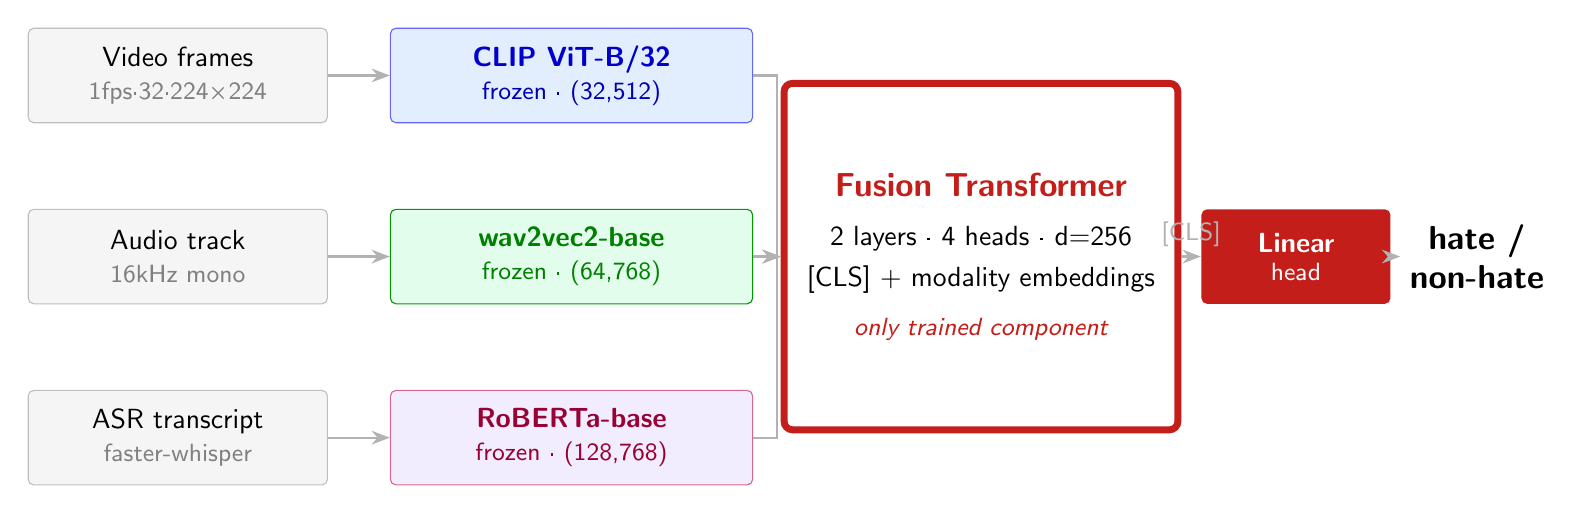
\begin{tikzpicture}[
      font=\normalsize,
      ibox/.style={draw=gray!50, fill=gray!8, rounded corners=2pt,
                   minimum width=38mm, minimum height=12mm, align=center},
      ebox/.style={draw,          rounded corners=2pt,
                   minimum width=46mm, minimum height=12mm, align=center},
      fbox/.style={draw=epflred, line width=2.5pt, rounded corners=3pt,
                   fill=white,   minimum width=50mm, minimum height=44mm,
                   align=center},
      hbox/.style={fill=epflred, rounded corners=2pt,
                   minimum width=24mm, minimum height=12mm, align=center},
      arr/.style={-Stealth, thick, gray!60},
    ]
      % Inputs
      \node[ibox] (vf) at ( 0,  2.3)
            {Video frames\\{\small\color{gray}1fps·32·224×224}};
      \node[ibox] (au) at ( 0,  0.0)
            {Audio track\\{\small\color{gray}16kHz mono}};
      \node[ibox] (tx) at ( 0, -2.3)
            {ASR transcript\\{\small\color{gray}faster-whisper}};

      % Encoders
      \node[ebox, fill=videobg!80,  draw=blue!60]         (clip) at (5.0,  2.3)
            {\textcolor{blue!80!black}{\bfseries CLIP ViT-B/32}\\
             {\small\color{blue!70!black}frozen · (32,512)}};
      \node[ebox, fill=audiobg!80,  draw=green!60!black]  (w2v)  at (5.0,  0.0)
            {\textcolor{green!50!black}{\bfseries wav2vec2-base}\\
             {\small\color{green!50!black}frozen · (64,768)}};
      \node[ebox, fill=textpurbg!80,draw=purple!60]       (rob)  at (5.0, -2.3)
            {\textcolor{purple!80!black}{\bfseries RoBERTa-base}\\
             {\small\color{purple!80!black}frozen · (128,768)}};

      % Fusion
      \node[fbox] (fus) at (10.2, 0.0)
            {\textcolor{epflred}{\large\bfseries Fusion Transformer}\\[2mm]
             2 layers · 4 heads · d=256\\[1mm]
             {[CLS] + modality embeddings}\\[2mm]
             {\small\itshape\color{epflred}only trained component}};

      % Head + output
      \node[hbox] (head) at (14.2, 0.0)
            {\bfseries\color{white}Linear\\[-2pt]
             \small\color{white!80}head};
      \node[align=center,font=\large\bfseries] (out) at (16.5, 0.0)
            {hate /\\ non-hate};

      % Arrows
      \draw[arr] (vf)--(clip);
      \draw[arr] (au)--(w2v);
      \draw[arr] (tx)--(rob);
      \draw[arr] (clip.east)--++(0.3,0)|-(fus.west);
      \draw[arr] (w2v.east)--(fus.west);
      \draw[arr] (rob.east)--++(0.3,0)|-(fus.west);
      \draw[arr] (fus.east)--
            node[above,font=\small\color{gray}]{[CLS]}
            (head.west);
      \draw[arr] (head)--(out);
    \end{tikzpicture}
    \par
  \end{pbox}

  \vspace{5mm}

  % ────────────────────────────────────────
  %  RELATED WORK
  % ────────────────────────────────────────
  \begin{pbox}{Related Work}
    \begin{itemize}[leftmargin=7mm, itemsep=3mm]
      \item \textbf{HateMM [1]} --- defines the task; releases the dataset
            and the community labels we audit against.
      \item \textbf{CLIP [2]} --- our frozen vision encoder; originally
            trained to match images with natural-language captions.
      \item \textbf{Attention Bottlenecks [3]} --- motivates our
            cross-modal fusion design; we use a lighter
            [CLS]-readout variant suited to this dataset scale.
    \end{itemize}
  \end{pbox}

  \vspace{5mm}

  % ────────────────────────────────────────
  %  REFERENCES
  % ────────────────────────────────────────
  \noindent{\color{epflred}\rule{\linewidth}{1pt}}
  \vspace{3mm}

  {\LARGE\bfseries\textcolor{epflred}{References}}
  \vspace{3mm}

  \begin{enumerate}[leftmargin=7mm, itemsep=3mm, font=\large]
    \item M.\ Das et al., ``HateMM: A Multi-Modal Dataset for Hate
          Video Classification,'' \emph{AAAI ICWSM}, vol.~17, 2023,
          pp.~1014--1023.
    \item A.\ Radford et al., ``Learning Transferable Visual Models
          From Natural Language Supervision,'' \emph{ICML}, vol.~139,
          2021, pp.~8748--8763.
    \item A.\ Nagrani et al., ``Attention Bottlenecks for Multimodal
          Fusion,'' \emph{NeurIPS}, vol.~34, 2021, pp.~14200--14213.
  \end{enumerate}

\end{minipage}%   ← end LEFT COLUMN
\hfill
% ─────────────────────────────────────────────────────────
\begin{minipage}[t]{0.465\textwidth}

  % ────────────────────────────────────────
  %  RESULTS
  % ────────────────────────────────────────
  \begin{pbox}{Results}
    {\large\color{gray}
     Test set · seed 42 · n\,=\,109 videos held out from training.
     Higher is better for all metrics.
     \colorbox{fusionrow}{\textcolor{epflred}{\bfseries Fusion}}
     uses all three modalities.}

    \vspace{5mm}
    {\Large\bfseries Table 1 --- Full modality ablation (seed 42, n\,=\,109).
    Bimodal rows: results in progress.}\\[3mm]

    % ── Table 1: modality ablation ──
    % Bimodal rows: replace --- with numbers once runs finish.
    % To update all numbers: search \% in this block and edit.
    \definecolor{birow}{RGB}{249,249,249}
    \renewcommand{\arraystretch}{1.4}
    {\large
    \begin{tabular}{lrrrrr}
      \toprule
      \textbf{Model}
        & \textbf{Acc.} & \textbf{F1}
        & \textbf{Prec.} & \textbf{Rec.} & \textbf{AUROC} \\
      \midrule
      \rowcolor{fusionrow}
      \textbf{\textcolor{epflred}{Fusion (V+A+T)}}
        & \textbf{\textcolor{epflred}{83.5\%}}
        & \textbf{\textcolor{epflred}{82.4\%}}
        & \textbf{\textcolor{epflred}{82.1\%}}
        & \textbf{\textcolor{epflred}{74.4\%}}
        & \textbf{\textcolor{epflred}{87.3\%}} \\
      \rowcolor{birow}
      \textit{\textcolor{gray}{Video+Text}}
        & \textit{\textcolor{gray}{---}}
        & \textit{\textcolor{gray}{---}}
        & \textit{\textcolor{gray}{---}}
        & \textit{\textcolor{gray}{---}}
        & \textit{\textcolor{gray}{---}} \\
      \rowcolor{birow}
      \textit{\textcolor{gray}{Audio+Text}}
        & \textit{\textcolor{gray}{---}}
        & \textit{\textcolor{gray}{---}}
        & \textit{\textcolor{gray}{---}}
        & \textit{\textcolor{gray}{---}}
        & \textit{\textcolor{gray}{---}} \\
      \rowcolor{birow}
      \textit{\textcolor{gray}{Video+Audio}}
        & \textit{\textcolor{gray}{---}}
        & \textit{\textcolor{gray}{---}}
        & \textit{\textcolor{gray}{---}}
        & \textit{\textcolor{gray}{---}}
        & \textit{\textcolor{gray}{---}} \\
      Text only  & 78.0\% & 76.3\% & 75.7\% & 65.1\% & 84.2\% \\
      Video only & 74.3\% & 72.6\% & 69.2\% & 62.8\% & 81.5\% \\
      Audio only & 69.7\% & 69.5\% & 58.9\%
                 & \textbf{76.7\%} & 77.5\% \\
      \bottomrule
    \end{tabular}}

    \vspace{6mm}

    % ── Bar chart image ──
    % Replace bar_chart.png to update the figure.
    \begin{center}
      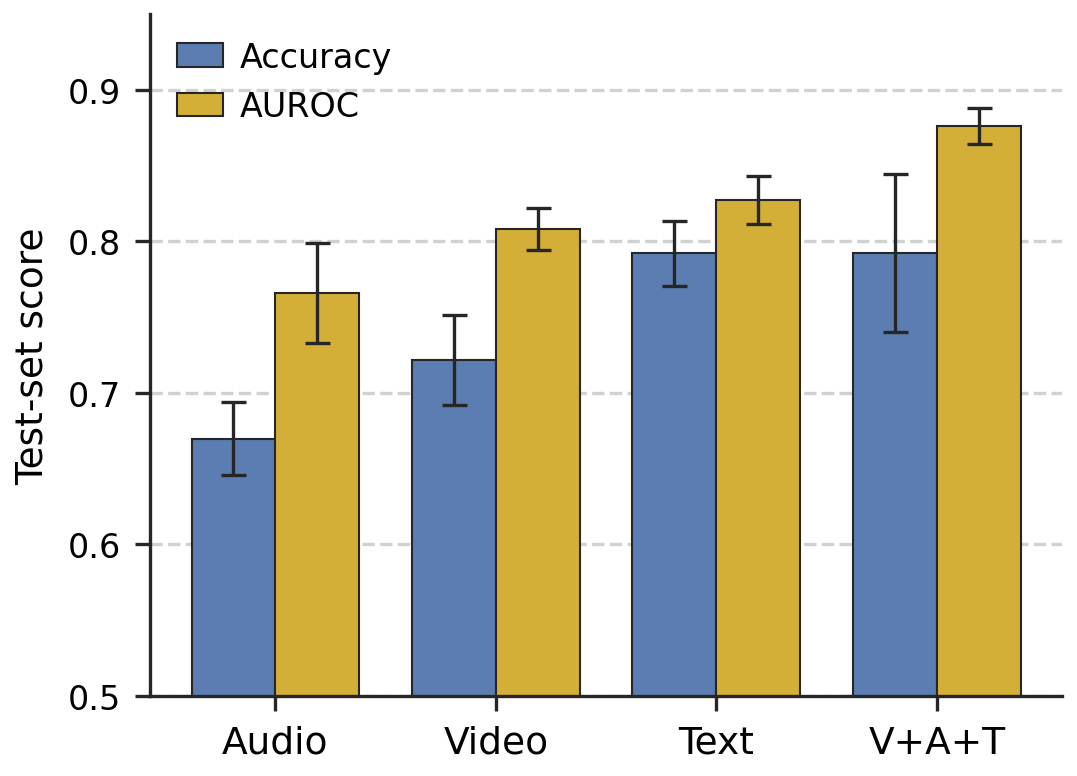
\includegraphics[width=\linewidth, height=55mm, keepaspectratio]
                      {bar_chart.png}\\[2mm]
      {\large\color{gray}
       Figure 1. Macro-F1 per model.
       Combining all three modalities (red bar) beats every single-sense baseline.}
    \end{center}

    \vspace{4mm}

    % ── Key observations ──
    \begin{obsbox}
      {\Large\bfseries\textcolor{epflred}{Key Observations}}
      \vspace{3mm}
      \begin{itemize}[leftmargin=6mm, itemsep=3mm]
        \item \textbf{Fusion wins on every metric.}
              +5.1\,pts accuracy, +6.1\,pts F1, +3.1\,pts AUROC over
              text-only. AUROC (ranking quality) shows the most
              reliable gain.
        \item \textbf{Text is the strongest single modality.}
              Most hate here is verbal. Yet text alone misses cases
              where the hate lies in tone or imagery.
        \item \textbf{Audio catches the most positives but is imprecise.}
              Highest recall (76.7\%), but precision is only 58.9\%
              --- it flags too many innocent videos.
      \end{itemize}
    \end{obsbox}
  \end{pbox}

  \vspace{5mm}

  % ────────────────────────────────────────
  %  FAIRNESS
  % ────────────────────────────────────────
  \begin{pbox}{Fairness: Does It Work for Everyone?}
    {\large
    The overall numbers look strong --- but does the model protect
    all communities equally?
    We break down accuracy for the three largest groups.}

    \vspace{5mm}
    {\Large\bfseries Table 2 --- Per-community accuracy (seed 42).}\\[3mm]

    % ── Table 2: per-community ──
    \renewcommand{\arraystretch}{1.4}
    {\large
    \begin{tabular}{lccccc}
      \toprule
      \textbf{Group} & \textbf{n}
        & \textbf{Fusion} & \textbf{Text}
        & \textbf{Video}  & \textbf{Audio} \\
      \midrule
      Blacks & 46
        & \textbf{\textcolor{epflred}{80.4\%}}
        & 71.7\% & 71.7\% & 63.0\% \\
      Jews   & 15
        & \textbf{\textcolor{epflred}{86.7\%}}
        & 73.3\% & 60.0\% & 73.3\% \\
      Others & 39
        & 84.6\%
        & \textbf{\textcolor{epflred}{87.2\%}}
        & 79.5\% & 71.8\% \\
      \bottomrule
    \end{tabular}}

    \vspace{5mm}

    % ── Bias callout (dark box) ──
    \begin{darkbox}
      \begin{minipage}[c]{0.07\linewidth}
        {\LARGE\bfseries\textcolor{yellow}{!}}
      \end{minipage}%
      \begin{minipage}[c]{0.90\linewidth}
        {\Large\bfseries\textcolor{warnred}{Hidden Bias in the ``Others'' Group}}\\[2mm]
        {\large\color{white!90}
        ``Others'' accuracy looks fine (84.6\%) --- but the
        \textbf{\textcolor{warnred}{F1 score is only 45.8\%}}.
        The model mostly predicts ``non-hate'' for this group and gets
        lucky because most ``Others'' videos are non-hateful.
        The actual hate videos in this group slip through.\\[2mm]
        \textbf{\textcolor{warnred}{High accuracy $\neq$ fair detection.}}
        Per-community F1 is the right metric to audit.}
      \end{minipage}
    \end{darkbox}
  \end{pbox}

  \vspace{5mm}

  % ────────────────────────────────────────
  %  LIMITATIONS
  % ────────────────────────────────────────
  \begin{pbox}{Limitations}
    \begin{itemize}[leftmargin=7mm, itemsep=3mm]
      \item \textbf{Small test set (n\,=\,109).}
            Per-community estimates carry high variance, especially
            for Jews (n\,=\,15: one video changes the score by 7\%).
      \item \textbf{Frozen backbones cap performance.}
            Intentional design for fair modality comparison.
            Fine-tuning the encoders would likely improve all rows.
      \item \textbf{ASR quality varies.}
            faster-whisper degrades on shouted speech, background music,
            and strong accents, weakening the text signal on a subset.
      \item \textbf{Class imbalance (60\% non-hate).}
            The model is conservative. We do not apply loss weighting
            to correct for this.
    \end{itemize}
  \end{pbox}

  \vspace{5mm}

  % ────────────────────────────────────────
  %  CONCLUSION
  % ────────────────────────────────────────
  \begin{pbox}{Conclusion}
    Combining sight, sound, and speech through a small Transformer
    \textbf{consistently beats every single-modality baseline} on hate
    video detection.
    The most robust gain is in ranking quality (+3.1\,pts AUROC over
    text-alone).
    False positives drop from 24\% (text only) to 18\% (fusion).

    \vspace{4mm}
    \clabel{Practical takeaway:}
    For content moderation pipelines that rank videos by risk,
    fusion is the clear choice.
    For a simple binary filter with limited compute,
    text-alone is strong and cheaper.
    In both cases, \emph{per-community F1 auditing is essential} ---
    accuracy alone can hide that certain groups are not being protected.
  \end{pbox}

\end{minipage}  % ← end RIGHT COLUMN

% ═════════════════════════════════════════════════════════
%  FOOTER
% ═════════════════════════════════════════════════════════
\vfill
\noindent{\color{gray!40}\rule{\textwidth}{0.5pt}}\\[2mm]
\centering{\large\color{gray}
  EE-559 Deep Learning \quad\textbullet\quad EPFL, Spring 2026}

\end{document}
